\chapter{الكواشف العضوية المغنيزيومية}\label{ch:b1:organomagnesium}

لمعظم الجزيئات العضوية المفيدة ذرات كربون أكثر مما في أي
مادة أولية رخيصة، والمشكلة المركزية في التخليق هي وصل هيكلين
كربونيين برابطة C--C جديدة. وفي المركب الكربوني يكون الكربون
في الغالب الطرفَ الفقير بالإلكترونات في الرابطة --- مع الأكسجين، أو مع
هالوجين --- وذرتا كربون فقيرتان بالإلكترونات لا تتفاعلان إحداهما مع الأخرى.
وفي مطلع القرن العشرين قلب هذا الوضعَ كاشفٌ يُحضَّر في دورق واحد من
هالوجينو ألكان والمغنيزيوم: فكربونه غني بالإلكترونات،
\omterm{def:b1:electronic-effects:nucleophile}{محب للنواة} يهاجم كربون مجموعة كربونيل. وبه يمكن
بناء كحولات ذات هياكل شبه اعتباطية من قطع أصغر. يبيّن هذا
الفصل كيف يُحضَّر الكاشف، ولماذا يحتاج إلى دورق جاف تمامًا،
وعلامَ يُضاف، وكيف يُخطَّط به.

\begin{recall}
\omterm{def:b1:periodicity:electronegativity}{الكهرسلبية} (\cref{ch:b1:periodicity})؛ وأحماض لويس وقواعده
والرابطة التساندية (\cref{ch:b1:lewis-resonance-vsepr})؛ \omterm{def:b1:electronic-effects:nucleophile}{والمحبات للنواة}،
\omterm{def:b1:electronic-effects:nucleophile}{والمحبات للإلكترونات}، \omterm{def:b1:electronic-effects:curly-arrow}{والأسهم المنحنية} وسلّم $\mathrm{p}K_a$ للأنواع
العضوية (\cref{ch:b1:electronic-effects})؛ وصنف الكحول
(أولي، ثانوي، ثالثي) يتبع صنف كربونه.
\end{recall}

\section{تحضير كاشف غرينيار}

\begin{definition}[المركب العضوي الفلزي، كاشف غرينيار]\label{def:b1:organomagnesium:organometallic}
\emph{المركب العضوي الفلزي}\index{مركب عضوي فلزي} يحتوي
رابطة كربون--فلز واحدة على الأقل. و\emph{المركب العضوي
المغنيزيومي}\index{مركب عضوي مغنيزيومي} فيه رابطة C--Mg؛
و\emph{كاشف غرينيار}\index{كاشف غرينيار} \ce{RMgX} (X = Cl، Br، I)،
المحضَّر من هالوجينو ألكان أو هالوجينو أرين والمغنيزيوم في إيثر،
\ce{R-X + Mg -> R-MgX}، هو الأكثر شيوعًا.
\end{definition}

يُدرج المغنيزيوم نفسه في الرابطة C--X. والإيثر ليس
مذيبًا بريئًا: فللمغنيزيوم في \ce{RMgX} أربعة \omterm{def:b1:quantum-numbers:configuration}{إلكترونات تكافؤ} فقط
حوله، ويعطيه جزيئا إيثر زوجيهما الحرين، فيكتمل
ثمانيه ويبقى الكاشف في المحلول.

\begin{omfigure}
\begin{tikzpicture}[font=\small]
  \node (mg) at (0,0) {Mg};
  \node (r) at (-1.5,0) {R};
  \node (x) at (1.5,0) {Br};
  \node (o1) at (0,1.45) {O};
  \node (o2) at (0,-1.45) {O};
  \draw[thick] (r) -- (mg) -- (x);
  \draw[thick, ->, omDef] (o1) -- (mg);
  \draw[thick, ->, omDef] (o2) -- (mg);
  \draw (o1) -- ++(-0.8,0.45) node[left] {\ce{CH3CH2}};
  \draw (o1) -- ++(0.8,0.45) node[right] {\ce{CH2CH3}};
  \draw (o2) -- ++(-0.8,-0.45) node[left] {\ce{CH3CH2}};
  \draw (o2) -- ++(0.8,-0.45) node[right] {\ce{CH2CH3}};
  \node[align=left, anchor=west] at (3.2,0) {جزيئا إيثر يعطي كل منهما\\\foreignlanguage{arabic}{زوجًا حرًا، بالأزرق:}\\\foreignlanguage{arabic}{مغنيزيوم رباعي الأوجه،}\\ثمانية إلكترونات};
\end{tikzpicture}

{\small \omterm{def:b1:organomagnesium:organometallic}{كاشف غرينيار} في الإيثوكسي إيثان (ثنائي إيثيل الإيثر).
والروابط التساندية أكسجين--مغنيزيوم تفسّر لماذا لا يتكوّن الكاشف إلا في
إيثر أو في \omterm{def:b1:lewis-resonance-vsepr:lewis-acid}{قاعدة لويس} مماثلة.}
\end{omfigure}

\begin{method}[تحضير كاشف غرينيار]\label{met:b1:organomagnesium:prepare}
\begin{enumerate}
  \item جفّف الأدوات الزجاجية كلها في فرن؛ وزوّد المكثف بأنبوب
        تجفيف بكلوريد الكالسيوم؛ واستعمل إيثرًا لامائيًا.
  \item ضع برادة المغنيزيوم وقليلًا من الإيثر في دورق ثلاثي الفتحات
        مزوّد بمكثف وقمع إضافة ومحرّك.
  \item أضف جزءًا صغيرًا من الهاليد؛ وحين يبدأ التفاعل
        (تعكّر، وغليان لطيف للإيثر)، أضف الباقي قطرةً قطرة
        بمعدل يحافظ على ارتداد لطيف.
  \item استعمل المحلول فورًا، في الجهاز الجاف نفسه.
\end{enumerate}
\end{method}

\begin{omfigure}
\begin{tikzpicture}[font=\small]
  \pic at (0,-0.05) {stirrer};
  \pic (f) at (0,0.05) {threeneck={0.35}{omDef!14}};
  \pic at (f-c) {condenser};
  \pic at ($(f-c)+(0,3.2)$) {guardtube};
  \pic[rotate=25] at (f-l) {dropfunnel={0.5}{orange!20}};
  \fill[black!45, rotate around={-25:(f-r)}] ($(f-r)+(-0.17,0)$) rectangle ++(0.34,0.3);
  \draw[->] (2.4,0.9) node[right] {\foreignlanguage{arabic}{برادة \babelsublr{Mg} في إيثر جاف}} -- (0.6,0.6);
  \draw[->] (-3.0,3.9) node[left, align=right] {\foreignlanguage{arabic}{الهاليد في الإيثر،}\\يُضاف قطرةً قطرة} -- (-1.8,3.4);
  \draw[->] (1.8,5.3) node[right] {مكثف مبرَّد بالماء} -- (0.45,4.8);
  \draw[->] (1.8,6.6) node[right] {أنبوب تجفيف بكلوريد الكالسيوم} -- (0.3,6.4);
  \draw[->] (2.4,-0.2) node[right] {محرّك مغناطيسي} -- (1.3,-0.2);
\end{tikzpicture}

{\small جهاز تفاعل غرينيار: كل ما يمكن أن يبلغه الهواء
مجفَّف. يوقف أنبوبُ التجفيف بخارَ ماء الهواء؛ ويعيد
المكثفُ الإيثرَ المغلي إلى الدورق.}
\end{omfigure}

\begin{inthelab}[تفاعل لا بد أن يبدأ]
يرفض تحضير غرينيار أحيانًا أن يبدأ: إذ يكون المغنيزيوم
مغطى بغشاء من الأكسيد. وسحق قطعة من البرادة بقضيب زجاجي، أو إضافة
\omterm{def:b1:crystals-metals:crystal}{بلورة} من اليود، أو تسخين الدورق موضعيًا يكشف فلزًا جديدًا.
وما إن يبدأ التفاعل حتى يصير ناشرًا للحرارة ويغلي الإيثر من تلقاء نفسه؛
فتُبطأ الإضافة عندئذ كي لا يفيض. والإيثوكسي إيثان
يغلي عند \qty{35}{\celsius} وبخاره شديد الاشتعال: فلا لهب
في أي مكان من المختبر، وحمام ثلج في متناول اليد.
% ledger: bp:diethylether
\end{inthelab}

\section{قاعدة قوية ومحب للنواة}

\begin{definition}[انقلاب القطبية]\label{def:b1:organomagnesium:umpolung}
\omterm{def:b1:periodicity:electronegativity}{كهرسلبية} المغنيزيوم (1.31) أدنى بكثير من \omterm{def:b1:periodicity:electronegativity}{كهرسلبية}
الكربون (2.55): ففي \ce{R-MgX} تكون الرابطة C--Mg مستقطبة وطرفها السالب
على الكربون، الذي يسلك سلوك \omterm{def:b1:electronic-effects:intermediates}{أنيون كربوني}. أما في الهاليد \ce{R-X} فكان
الكربون نفسه موجبًا (X: 2.96 للبروم). وتحويل كربون \omterm{def:b1:electronic-effects:nucleophile}{محب للإلكترونات}
إلى كربون \omterm{def:b1:electronic-effects:nucleophile}{محب للنواة} هو \emph{انقلاب القطبية}\index{انقلاب القطبية}.
% ledger: en:Mg, en:C, en:Br
\end{definition}

\begin{proposition}[الهيدروجينات الحمضية تهدم كواشف غرينيار]\label{prop:b1:organomagnesium:base}
يتفاعل \omterm{def:b1:organomagnesium:organometallic}{كاشف غرينيار} تفاعلًا كميًا مع الماء، والكحولات، والأحماض
الكربوكسيلية، والأمينات ذات الروابط N--H والألكاينات الطرفية، فيعطي الألكان
\ce{R-H}: \ce{RMgX + H2O -> R-H + Mg(OH)X}.
\end{proposition}

\begin{proof}
الكربون الشبيه \omterm{def:b1:electronic-effects:intermediates}{بالأنيون الكربوني} هو قاعدة المزدوجة $\ce{R-H}/\ce{R^-}$،
والألكانات أضعف الأحماض في الكيمياء العضوية إلى حد بعيد: فلا يمكن
قياس مغادرة أي بروتون منها في الماء، حيث الهيدروكسيد أقوى قاعدة
يمكن أن توجد (\cref{ch:b1:predominant-reaction}، التسوية). وأي حمض
في القائمة أقوى بكثير، ولانتقال البروتون إلى \ce{R^-}
ثابت هائل: فهو تام وسريع.
\end{proof}

وهذا سبب الجهاز الجاف: فقطرة ماء تهدم كمية
مساوية من الكاشف. وإذا حُوّل ذلك إلى ميزة، فإن \ce{CH3CH2MgBr + D2O}
يضع ذرة دوتيريوم في موضع البروم بالضبط.

\section{الإضافة إلى مركبات الكربونيل وثنائي أكسيد الكربون}

كربون المجموعة C=O \omterm{def:b1:electronic-effects:nucleophile}{محب للإلكترونات}
(\cref{ch:b1:electronic-effects}). ويضيف \omterm{def:b1:organomagnesium:organometallic}{كاشف غرينيار} مجموعته R
إليه، فيذهب زوج $\pi$ للرابطة C=O إلى الأكسجين؛ ثم تبرتن معالجةٌ
حمضية الألكوكسيدَ.

\begin{omfigure}
\setchemfig{atom sep=2.1em}
\schemestart
\chemfig{@{r}R-[@{rm}]MgBr}
\+
\chemfig{@{cc}C(-[:150]R')(-[:210]R'')=[@{co}]@{o}O}
\arrow{->}
\chemfig{C(-[:150]R')(-[:210]R'')(-[2]R)-O^{-}}
\chemfig{\phantom{.}}\chemfig{^{+}MgBr}
\arrow{->[\ce{H3O+}]}
\chemfig{C(-[:150]R')(-[:210]R'')(-[2]R)-OH}
\schemestop
\chemmove{\draw[->, thick, shorten <=2pt, shorten >=2pt](rm) .. controls +(70:9mm) and +(180:7mm) .. (cc);
          \draw[->, thick, shorten <=2pt, shorten >=2pt](co) .. controls +(90:6mm) and +(90:6mm) .. (o);}
\par\vspace{6pt}

{\small إضافة \omterm{def:b1:organomagnesium:organometallic}{كاشف غرينيار} إلى كيتون (أو إلى ألدهيد،
$\mathrm{R''} = \mathrm{H}$): يكوّن زوج C--Mg الرابطة C--C الجديدة بينما يذهب زوج $\pi$
للرابطة C=O إلى الأكسجين؛ ويُبرتَن ألكوكسيد المغنيزيوم بحمض مخفف
في خطوة منفصلة.}
\end{omfigure}

\begin{proposition}[الكحولات من مركبات الكربونيل]\label{prop:b1:organomagnesium:carbonyl-addition}
بعد المعالجة الحمضية، يعطي \omterm{def:b1:organomagnesium:organometallic}{كاشف غرينيار} \ce{RMgX}: مع الميثانال،
كحولًا أوليًا \ce{RCH2OH}؛ ومع ألدهيد آخر $\mathrm{R'CHO}$، كحولًا
ثانويًا $\mathrm{RR'CHOH}$؛ ومع كيتون $\mathrm{R'COR''}$، كحولًا ثالثيًا
$\mathrm{RR'R''COH}$. وتصل الرابطة C--C الجديدة R بكربون الكربونيل السابق.
\end{proposition}

\begin{proof}
يحتفظ كربون الكربونيل بمتبادليه ويكتسب R ومجموعة OH
(من أكسجين الألكوكسيد): فالميثانال يجلب ذرتي H، والألدهيد ذرة H واحدة
ومجموعة كربونية واحدة، والكيتون مجموعتين كربونيتين. وصنف الكحول هو
عدد المجموعات الكربونية على ذلك الكربون: واحدة أو اثنتان أو ثلاث.
\end{proof}

\begin{proposition}[الأحماض الكربوكسيلية من ثنائي أكسيد الكربون]\label{prop:b1:organomagnesium:co2}
\omterm{def:b1:organomagnesium:organometallic}{كاشف غرينيار} المسكوب على ثنائي أكسيد الكربون الصلب يعطي، بعد
التحميض، الحمض الكربوكسيلي \ce{RCOOH} بكربون إضافي:
\ce{RMgX + CO2 -> RCOOMgX}، ثم \ce{RCOOMgX + H3O+ -> RCOOH + Mg^2+ + X- + H2O}.
\end{proposition}

\begin{proof}
\ce{CO2} مركب كربونيلي يُهاجَم كربونه كما يُهاجَم كربون
الكيتون؛ والكربوكسيلات المتكوّنة أضعف تفاعليةً من أن تضيف مجموعة R ثانية
في هذه الظروف (فالكربونيل المشحون سلبًا \omterm{def:b1:electronic-effects:nucleophile}{محب
للإلكترونات} ضعيف). ويبرتنها الحمض.
\end{proof}

\section{بناء الهياكل الكربونية}

\begin{method}[التخطيط لكحول]\label{met:b1:organomagnesium:plan-alcohol}
\begin{enumerate}
  \item عيّن الكربون الحامل لمجموعة OH في الكحول المستهدف.
  \item اختر إحدى مجموعاته الكربونية لتكون R (ستأتي من
        \omterm{def:b1:organomagnesium:organometallic}{كاشف غرينيار}، المحضَّر من \ce{R-Br})؛ وبقية
        الجزيء، مع ذلك الكربون على هيئة C=O، هو الشريك الكربونيلي.
  \item اذكر الخيارات الممكنة (خيار لكل مجموعة كربونية) وفضّل
        الخيار ذا الكواشف البسيطة المتاحة.
  \item تحقق من أن أيًّا من الشريكين لا يحمل هيدروجينًا حمضيًا أو مجموعة كربونيل
        ثانية قد تتفاعل هي أيضًا.
\end{enumerate}
\end{method}

\begin{example}[2-فينيل بوتان-2-أول]\label{ex:b1:organomagnesium:plan}
يحمل الكربون الحامل لمجموعة OH مجموعة فينيل ومجموعة ميثيل ومجموعة إيثيل.
ثلاثة خيارات: بروميد فينيل المغنيزيوم مع البوتان-2-ون؛ وبروميد ميثيل المغنيزيوم
مع 1-فينيل بروبان-1-ون؛ وبروميد إيثيل المغنيزيوم مع
1-فينيل إيثان-1-ون (الأسيتوفينون). والثلاثة كلها تنجح؛ ويستعمل الأخير اثنين من
أكثر الكواشف شيوعًا.
\end{example}

\begin{history}[فيكتور غرينيار]
\begin{minipage}[t]{0.2\linewidth}\vspace{0pt}
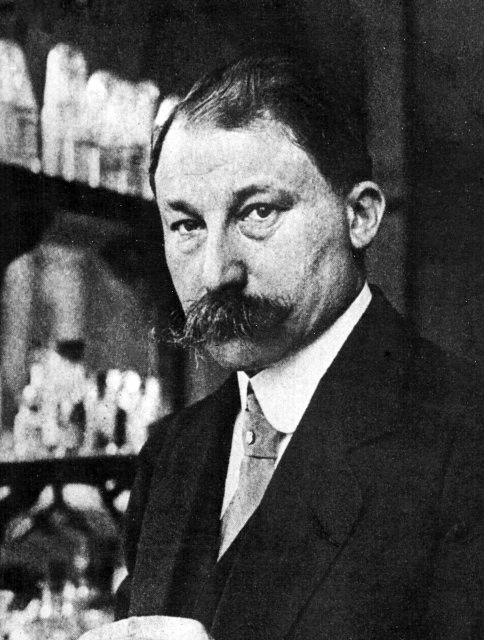
\includegraphics[width=\linewidth]{images/book2/grignard.jpg}
\end{minipage}\hfill
\begin{minipage}[t]{0.76\linewidth}\vspace{0pt}
يحمل الكاشف اسم فيكتور غرينيار، الذي وجد، وهو طالب دكتوراه
في مطلع القرن العشرين، أن المغنيزيوم يذوب في
محلول إيثري لهالوجينو ألكان وأن المحلول يُضاف إلى
مركبات الكربونيل. وجعلته بساطته --- فلز واحد، ومذيب واحد، ودورق واحد
--- أكثر تفاعلات تكوين الروابط كربون--كربون استعمالًا في
ذلك القرن، ونال بها مكتشفه جائزة نوبل في الكيمياء.
(صورة، ملكية عامة، ويكيميديا كومنز.)
\end{minipage}
\end{history}

\section{تمارين}

\begin{exercise}[$\star$]\label{exo:b1:organomagnesium:1}
اكتب تحضير بروميد إيثيل المغنيزيوم وتحضير
بروميد فينيل المغنيزيوم. وأعطِ استقطاب الرابطة C--Br واستقطاب
الرابطة C--Mg، مع الكهرسلبيات.
\end{exercise}

\begin{exercise}[$\star$]\label{exo:b1:organomagnesium:2}
ماذا يعطي يوديد ميثيل المغنيزيوم مع: الماء؛ والإيثانول؛ وحمض
الإيثانويك؛ وأكسيد الدوتيريوم \ce{D2O}؟ اكتب المعادلات.
\end{exercise}

\begin{exercise}[$\star$]\label{exo:b1:organomagnesium:3}
أعطِ الناتج (بعد المعالجة الحمضية) لبروميد إيثيل المغنيزيوم مع
الميثانال، والإيثانال، والبروبانون، والبنزالدهيد وثنائي أكسيد الكربون. وأعطِ
صنف كل كحول.
\end{exercise}

\begin{exercise}[$\star$]\label{exo:b1:organomagnesium:4}
لماذا يجب ألا يُستعمل 4-بروموبوتان-1-أول لتحضير \omterm{def:b1:organomagnesium:organometallic}{كاشف غرينيار}؟
\end{exercise}

\begin{exercise}[$\star\star$]\label{exo:b1:organomagnesium:5}
اكتب آلية إضافة بروميد ميثيل المغنيزيوم إلى الإيثانال
وآلية المعالجة، \omterm{def:b1:electronic-effects:curly-arrow}{بالأسهم المنحنية}. هل الناتج \omterm{def:b1:stereochemistry-in-depth:stereocentre}{كيرالي}؟ وهل
يُحصل عليه على هيئة \omterm{def:b1:stereochemistry-in-depth:enantiomers}{متماكب مرآوي} وحيد؟ ولماذا؟
\end{exercise}

\begin{exercise}[$\star\star$]\label{exo:b1:organomagnesium:6}
اقترح طريقتين لتحضير 3-ميثيل بنتان-3-أول من \omterm{def:b1:organomagnesium:organometallic}{كاشف غرينيار}
وكيتون.
\end{exercise}

\begin{exercise}[$\star\star$]\label{exo:b1:organomagnesium:7}
كيف تحضّر حمض 2-ميثيل البروبانويك من 2-بروموبروبان؟ احسب
كتلة الحمض المحصَّل عليها من \qty{12.3}{g} من البروميد \omterm{def:b1:extent-q-and-k:fractional-extent}{بمردود}
\qty{70}{\percent} ($M$: \ce{C3H7Br} \qty{123.0}{g/mol}، \ce{C4H8O2}
\qty{88.0}{g/mol}).
\end{exercise}

\begin{exercise}[$\star\star$]\label{exo:b1:organomagnesium:8}
يحضّر طالب مهمل بروميد فينيل المغنيزيوم من
\qty{0.0500}{mol} من البروموبنزين في إيثر يحتوي \qty{0.18}{g} من
الماء. ما كسر الكاشف الذي يُهدم؟ وأي ناتج يتكوّن؟
\end{exercise}

\begin{exercise}[$\star\star$]\label{exo:b1:organomagnesium:9}
ثنائي الفينيل، \ce{C6H5-C6H5}، ناتج جانبي لتحضير
بروميد فينيل المغنيزيوم. اقترح كيف يتكوّن، ولماذا تحدّ منه الإضافة البطيئة
للبروموبنزين إلى فائض من المغنيزيوم.
\end{exercise}

\begin{exercise}[$\star\star\star$]\label{exo:b1:organomagnesium:10}
خطّط لتخليقين للمركب 1-فينيل إيثان-1-أول من \omterm{def:b1:organomagnesium:organometallic}{كاشف غرينيار}، ولتخليق
للمركب 2-فينيل بروبان-2-أول. وسمِّ في كل حالة الهاليد الذي يعطي
الكاشف.
\end{exercise}

\begin{exercise}[$\star\star\star$]\label{exo:b1:organomagnesium:11}
فسّر لماذا يجب خلط \omterm{def:b1:organomagnesium:organometallic}{كاشف غرينيار} ومركب الكربونيل
بالترتيب المختار في المسألة أدناه، ولماذا تُجرى المعالجة
بحمض مخفف بارد لا بالماء وحده.
\end{exercise}

\begin{exercise}[$\star\star\star$]\label{exo:b1:organomagnesium:12}
يُعايَر \omterm{def:b1:organomagnesium:organometallic}{كاشف غرينيار} محضَّر من \qty{0.100}{mol} من بروميد:
فتُسكب عيّنة منه في فائض من الماء، ويُعاير ملح المغنيزيوم القاعدي
المتكوّن بحمض الهيدروكلوريك: وبالتحويل إلى المحلول كله،
يلزم \qty{0.088}{mol} من الحمض. اشرح المبدأ وأعطِ \omterm{def:b1:extent-q-and-k:fractional-extent}{مردود}
التحضير.
\end{exercise}

\section{مسألة: ثلاثي فينيل الميثانول}

\begin{problem}[{مسألة نهاية الأسبوع --- تحضير بروميد فينيل المغنيزيوم،
وإضافته إلى البنزوفينون، والمعالجة، ومردود
ثلاثي فينيل الميثانول}]
\label{pb:b1:organomagnesium:1}
في دورق ثلاثي الفتحات جاف، يعطي \qty{0.535}{g} من المغنيزيوم
و\qty{3.14}{g} من البروموبنزين في إيثوكسي إيثان لامائي
بروميدَ فينيل المغنيزيوم. ثم يُضاف قطرةً قطرة محلول من \qty{3.28}{g} من البنزوفينون،
\ce{(C6H5)2CO}، في الإيثر نفسه. وبعد المعالجة
بحمض الكبريتيك المخفف البارد، والاستخلاص وإعادة التبلور،
يُحصل على \qty{3.75}{g} من ثلاثي فينيل الميثانول النقي، \ce{(C6H5)3COH}،
ويُفصل \qty{0.15}{g} من ثنائي الفينيل. الكتل المولية (\unit{g/mol}):
Mg 24.3، \ce{C6H5Br} 156.9، \ce{C13H10O} 182.0، \ce{C19H16O} 260.0،
\ce{C12H10} 154.0، \ce{C7H6O2} 122.0.

\medskip
\noindent\textbf{الجزء الأول --- بروميد فينيل المغنيزيوم.}
\begin{enumerate}
  \item اكتب معادلة التحضير.
  \item احسب كميتي المغنيزيوم والبروموبنزين. أيهما
        بفائض؟
  \item لماذا يجب أن يكون الجهاز جافًا؟ اكتب التفاعل مع الماء.
  \item ما دور أنبوب التجفيف؟
  \item لماذا كان الإيثر أساسيًا، أبعد من إذابة الكواشف؟
  \item يأتي ثنائي الفينيل من تفاعل الكاشف مع البروموبنزين.
        اكتبه واحسب كمية البروموبنزين المفقودة بسببه.
\end{enumerate}

\medskip
\noindent\textbf{الجزء الثاني --- الإضافة.}
\begin{enumerate}[resume]
  \item احسب كمية البنزوفينون.
  \item اكتب آلية الإضافة \omterm{def:b1:electronic-effects:curly-arrow}{بالأسهم المنحنية}.
  \item أي كاشف يحدّ تكوّن ثلاثي فينيل الميثانول؟ خذ
        الجزء الأول في الحسبان.
  \item هل ثلاثي فينيل الميثانول \omterm{def:b1:stereochemistry-in-depth:stereocentre}{كيرالي}؟ علّل.
  \item لماذا يُضاف البنزوفينون إلى الكاشف، لا العكس؟
  \item ماذا كان سيفعل أثر من الماء في محلول البنزوفينون؟
\end{enumerate}

\medskip
\noindent\textbf{الجزء الثالث --- المعالجة.}
\begin{enumerate}[resume]
  \item اكتب برتنة الألكوكسيد.
  \item لماذا يُستعمل حمض مخفف بارد لا الماء وحده؟
  \item أين يوجد ثلاثي فينيل الميثانول وأملاح المغنيزيوم بعد
        الاستخلاص بالإيثر؟
  \item كيف يُفصل ثنائي الفينيل عن ثلاثي فينيل الميثانول؟ (ثنائي الفينيل أكثر
        \omterm{def:b1:precipitation:solubility}{ذوبانية} بكثير في إيثر البترول الخفيف البارد.)
  \item أي اختبار يؤكد نقاوة البلورات؟
  \item يصمد ثلاثي فينيل الميثانول أمام الحمض المخفف البارد، لكنه يذوب في
        حمض الكبريتيك المركّز فيعطي \omterm{def:b1:electronic-effects:intermediates}{كاتيونًا كربونيًا} أصفر داكنًا.
        اكتب تكوّنه وفسّر ثباته (قارن مع
        \cref{ch:b1:electronic-effects}).
\end{enumerate}

\medskip
\noindent\textbf{الجزء الرابع --- \omterm{def:b1:extent-q-and-k:fractional-extent}{المردود}، وناتج آخر.}
\begin{enumerate}[resume]
  \item احسب كمية ثلاثي فينيل الميثانول المحصَّل عليها.
  \item احسب \omterm{def:b1:extent-q-and-k:fractional-extent}{المردود} بالنسبة إلى الكاشف المحدِّد.
  \item اقترح سببين للفقد.
  \item لو سُكب كاشف الجزء الأول (مصحَّحًا بثنائي الفينيل) بدلًا من ذلك
        على ثنائي أكسيد الكربون الصلب، فأي ناتج كان سيتكوّن؟
  \item احسب الكتلة النظرية لذلك الناتج.
  \item اكتب معادلة تلك الكربوكسلة.
  \item اذكر \omterm{def:b1:extent-q-and-k:fractional-extent}{مردود} ثلاثي فينيل الميثانول، بالنسبة المئوية.
\end{enumerate}
\end{problem}
